\documentclass[aspectratio=169]{beamer}
\usetheme{Singapore}
\setbeamertemplate{caption}[numbered]
\addtobeamertemplate{navigation symbols}{}{%
    \usebeamerfont{footline}%
    \usebeamercolor[fg]{footline}%
    \hspace{1em}%
    \raisebox{1.4pt}[0pt][0pt]{\insertframenumber/\inserttotalframenumber}
}

\usefonttheme[onlymath]{serif}

\usepackage{cmap}
\usepackage[english]{babel}
\usepackage[T1]{fontenc}
\usepackage[utf8]{inputenc}
\usepackage[kerning=true]{microtype}
\usepackage{lmodern}

\usepackage{amsmath}
\usepackage{amsfonts}
\usepackage{amssymb}
\usepackage{amsthm}

\usepackage{mathtools}
\usepackage{wrapfig}
\usepackage{tikz}
\usepackage{xcolor}
\usetikzlibrary{positioning}

\usepackage[
    backend=biber,
    style=numeric,
]{biblatex}
\usepackage{graphicx}
\usepackage[justification=centering]{caption}
\usepackage{csquotes}

\graphicspath{{../images/}}

\addbibresource{../report/report.bib}
\renewcommand*{\bibfont}{\footnotesize}

\AtBeginSection[]
{
  \begin{frame}
    \frametitle{Plan}
    \tableofcontents[currentsection]
  \end{frame}
}


\theoremstyle{definition}
\newtheorem*{exemple}{Example}

\renewcommand{\leq}{\leqslant}
\renewcommand{\geq}{\geqslant}


\title{\textbf{Image Colorization and Upscaling using DC-GANs}}

\author{
    Nathan Frison\inst{1}\and Hubert Gruniaux\inst{1}\and Antoine Groudiev\inst{1}
}
\institute[shortinst]{\inst{1} École Normale Supérieure -- PSL\\\texttt{firstname.name@ens.psl.eu}}

\titlegraphic{
\includegraphics[height=1.6cm]{logo-ens-psl.png}}

\date{\today}

\begin{document}
\frame{\titlepage}

\begin{frame}{The image colorization problem}
    \begin{figure}
        \centering
        \begin{tikzpicture}
            \node at (0,0) {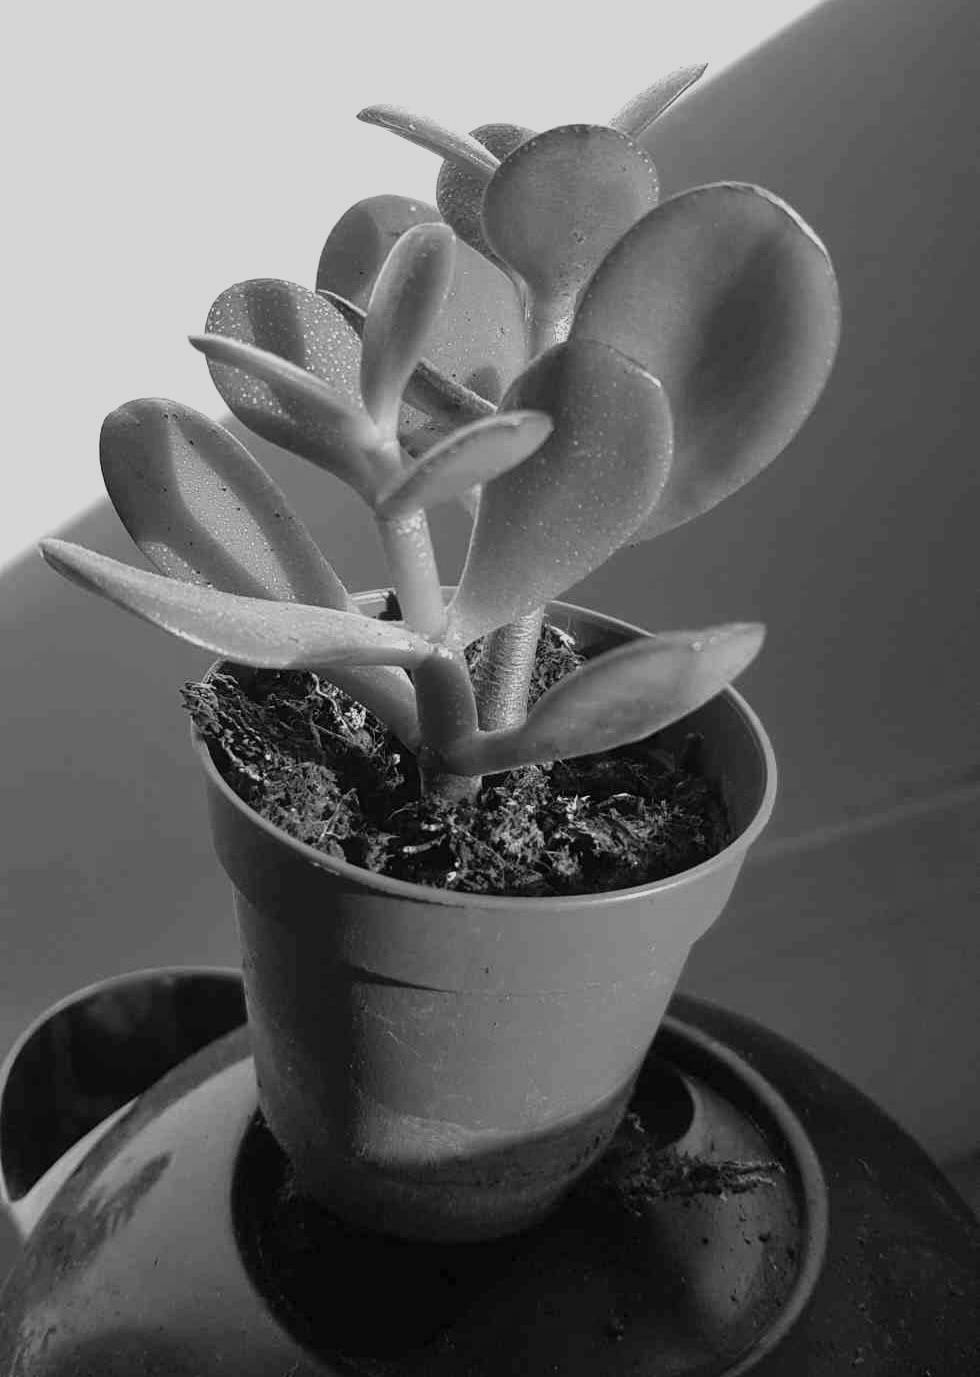
\includegraphics[width=.25\textwidth]{gray-plante.jpg}};
            \node at (0,-2.8) {Grayscale image};

            \draw[->, very thick] (2,-.2) -- ++(1,0);
            \draw[draw=black, thick, fill=orange!60, rounded corners] (3.2,-1.5) rectangle ++(3.5,2.5) node[pos=.5] {Neural Network};
            \draw[->, very thick] (7,-.2) -- ++(1,0);

            \node at (10,0) {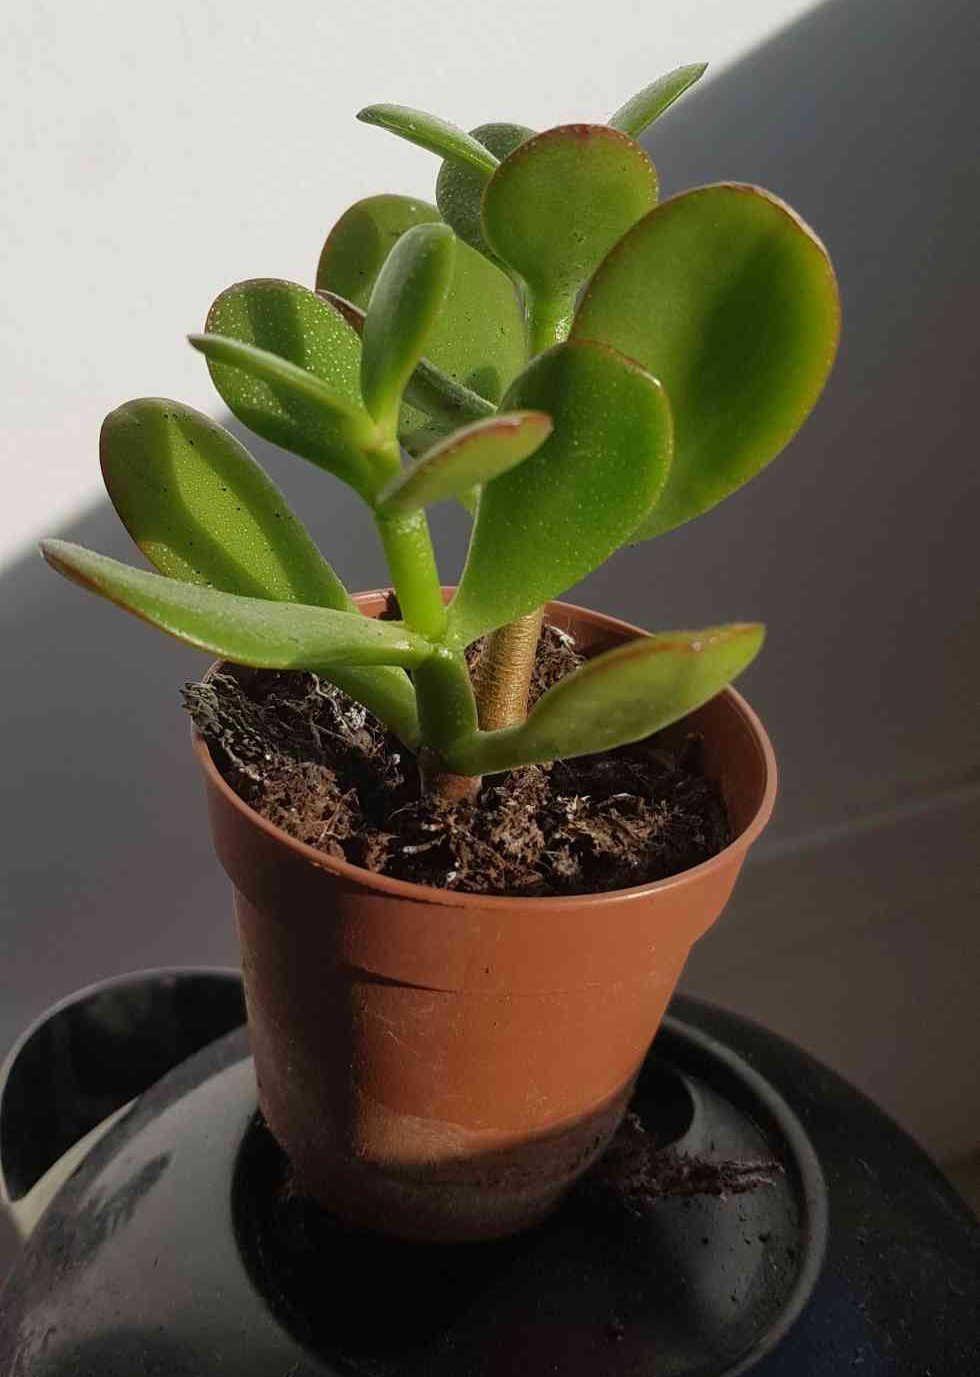
\includegraphics[width=.25\textwidth]{plante.jpg}};
            \node at (10,-2.8) {Colorized image};
        \end{tikzpicture}
    \end{figure}
\end{frame}

\begin{frame}{The image upscaling problem}
    \begin{figure}
        \centering
        \begin{tikzpicture}
            \node at (0,0) {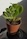
\includegraphics[width=.25\textwidth]{plante-low-res.jpg}};
            \node at (0,-2.8) {Low-resolution image};

            \draw[->, very thick] (2,-.2) -- ++(1,0);
            \draw[draw=black, thick, fill=orange!60, rounded corners] (3.2,-1.5) rectangle ++(3.5,2.5) node[pos=.5] {Neural network};
            \draw[->, very thick] (7,-.2) -- ++(1,0);

            \node at (10,0) {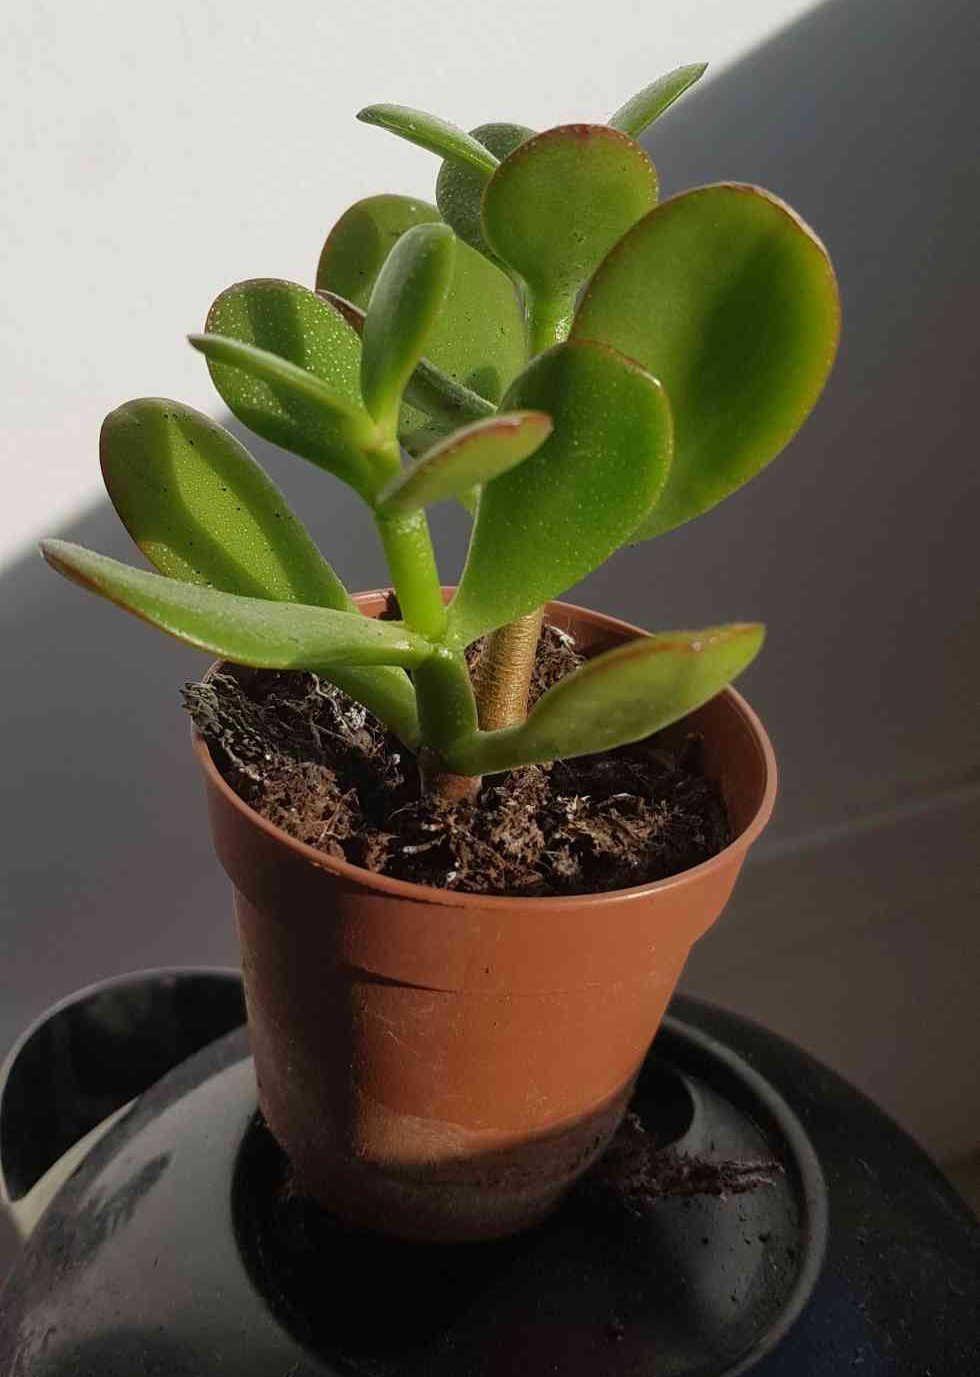
\includegraphics[width=.25\textwidth]{plante.jpg}};
            \node at (10,-2.8) {High-resolution image};
        \end{tikzpicture}
    \end{figure}
\end{frame}

\begin{frame}{Generative Adversarial Networks (GANs)}
    \begin{figure}
    \centering
    \begin{tikzpicture}[scale=.9]
        \draw[draw=black, thick, fill=gray!40, rounded corners] (0, -1) rectangle ++(1.3, 2.7) node[pos=.5] {$\begin{bmatrix}z_0\\z_1\\\dots\\z_n\end{bmatrix}$};
        \node at (0.8,-1.4) {Sample from $p_z$};

        \draw[->, very thick] (1.4,0.3) -- ++(1,0);
        \draw[draw=black, thick, fill=orange!60, rounded corners] (2.5, -.7) rectangle ++(3, 2) node[pos=.5] {Generator};
        \draw[->, very thick] (5.7,0.3) -- ++(.7,0);

        \node at (7.6,0.3) {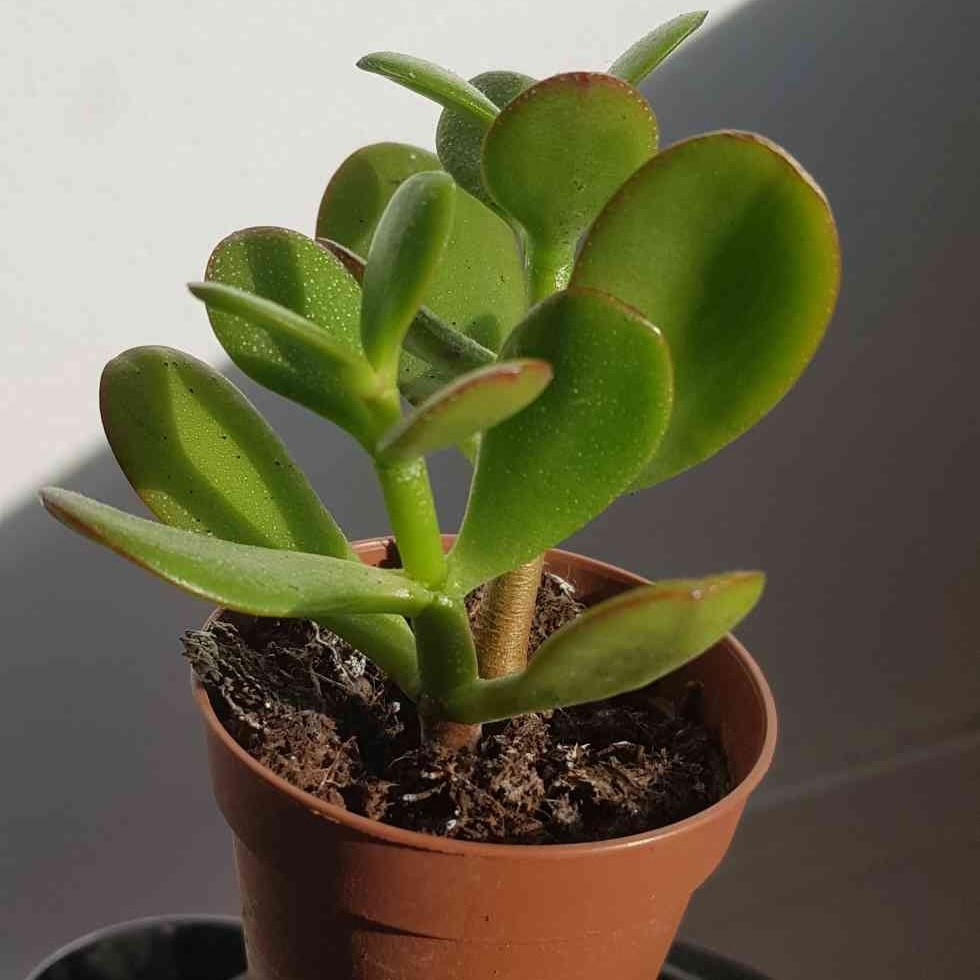
\includegraphics[width=1.8cm]{plante-sq.jpg}};
        \node at (7.6,1.6){Generated image};
        \node at (7.6,-2.5) {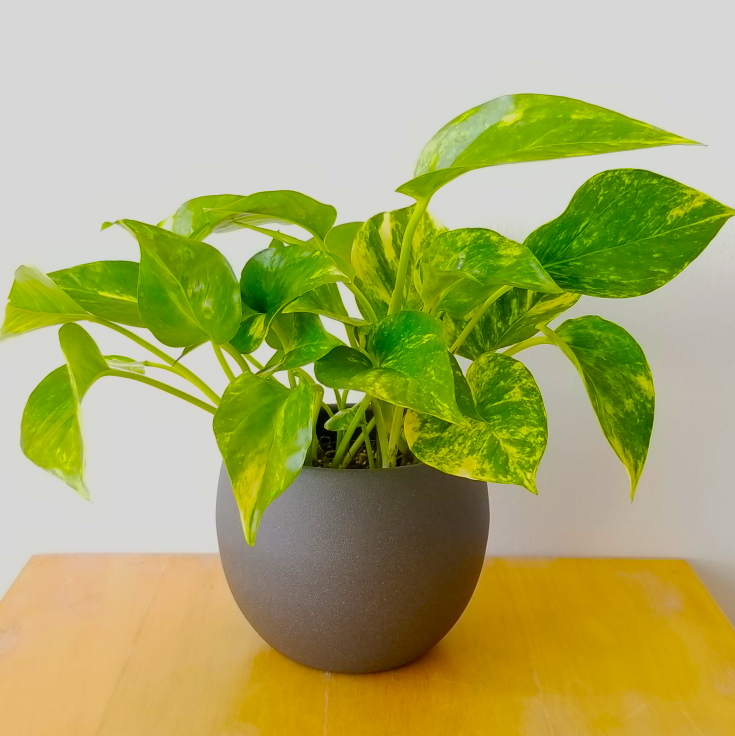
\includegraphics[width=1.8cm]{plante2.png}};
        \node at (7.6,-3.8){Dataset image};

        \draw[->, very thick] (8.7,0.3) -- ++(1,0);
        \draw[->, very thick] (8.7,-3.3) -- ++(.6,0) -- ++(0, 3.2) -- ++(.4, 0);
        
        \draw[draw=black, thick, fill=cyan!60, rounded corners] (10, -.7) rectangle ++(3, 2) node[pos=.5] {Discriminator};

        \draw[->, very thick] (13.1,.3) -- ++(.6,0) node[right] {$[0,1]$};
    \end{tikzpicture}
    \end{figure}
\end{frame}

\begin{frame}{Generative Adversarial Networks (GANs)}{Generation}
    \begin{itemize}
        \item The generator $G_{\theta_G}$ takes a random noise vector $z$ as input and outputs an image $G_{\theta_G}(z)$.
        \item The discriminator $D_{\theta_D}$ takes an image $x$ as input and outputs a probability $D_{\theta_D}(x)$ that the image is real.
        \item Minimax game problem:
        \begin{equation*}
            \min_{\theta_G}\max_{\theta_D} V(G_{\theta_G}, D_{\theta_D}) = \min_{\theta_G}\max_{\theta_D}\mathbb{E}_x[\log D_{\theta_D}(x)] + \mathbb{E}_z[\log(1 - D_{\theta_D}(G_{\theta_G}(z)))]
        \end{equation*}
    \end{itemize}
\end{frame}

\begin{frame}{Generative Adversarial Networks (GANs)}{Image colorization or upscaling}
    Change the generator to fit the colorization/upscaling problem using conditional GANs:
    \begin{itemize}
        \item Replace the noise vector $z$ by a grayscale/lows-res image $z$.
        \item The generator $G_{\theta_G}$ takes a grayscale/lows-res image $z$ as input and outputs an enhanced image $G_{\theta_G}(z)$.
        \item The discriminator receives both the enhanced image and the enhanced image (condition) as input, and outputs a probability $D_{\theta_D}(x|z)$ that the image is real.
    \end{itemize}
\end{frame}

\begin{frame}{Possible approaches}
    \begin{itemize}
        \item Colorize then upscale: train a colorization GAN and an upscaling GAN separately
        \item Upscale then colorize: train an upscaling GAN and a colorization GAN separately
        \item Joint training: train a single GAN to perform both tasks
    \end{itemize}
\end{frame}

\begin{frame}{References}
    \begin{enumerate}
        \item Goodfellow, I., Pouget-Abadie, J., Mirza, M., Xu, B., Warde-Farley, D., Ozair, S., ... \& Bengio, Y. (2014). Generative adversarial nets. \emph{Advances in neural information processing systems}, 27.
        \item Nazeri, Kamyar, Eric Ng, and Mehran Ebrahimi. "Image colorization using generative adversarial networks." \emph{Articulated Motion and Deformable Objects: 10th International Conference, AMDO 2018, Palma de Mallorca, Spain, July 12-13, 2018, Proceedings 10}. Springer International Publishing, 2018.
        \item Anwar, Saeed, et al. "Image colorization: A survey and dataset." \emph{Information Fusion} (2024): 102720.
        \item Wang, Xintao, et al. "Esrgan: Enhanced super-resolution generative adversarial networks." \emph{Proceedings of the European conference on computer vision (ECCV) workshops}. 2018.
    \end{enumerate}
\end{frame}

\end{document}